% ******************************************************** %
%              TEMPLATE DE INFORME ORGA2 v0.1              %
% ******************************************************** %
% ******************************************************** %
%                                                          %
% ALGUNOS PAQUETES REQUERIDOS (EN UBUNTU):                 %
% ========================================
%                                                          %
% texlive-latex-base                                       %
% texlive-latex-recommended                                %
% texlive-fonts-recommended                                %
% texlive-latex-extra?                                     %
% texlive-lang-spanish (en ubuntu 13.10)                   %
% ******************************************************** %


\documentclass[a4paper]{article}
\usepackage[spanish]{babel}
\usepackage[utf8]{inputenc}
\usepackage{charter}   % tipografia
\usepackage{graphicx}
%\usepackage{makeidx}
\usepackage{paralist} %itemize inline


%\usepackage{float}
%\usepackage{amsmath, amsthm, amssymb}
%\usepackage{amsfonts}
%\usepackage{sectsty}
%\usepackage{charter}
%\usepackage{wrapfig}
%\usepackage{listings}
%\lstset{language=C}

% \setcounter{secnumdepth}{2}
\usepackage{underscore}
\usepackage{caratula}
\usepackage{url}
\usepackage{ragged2e}


% ********************************************************* %
% ~~~~~~~~              Code snippets             ~~~~~~~~~ %
% ********************************************************* %

\usepackage{color} % para snipets de codigo coloreados
\usepackage{fancybox}  % para el sbox de los snipets de codigo

\definecolor{litegrey}{gray}{0.94}

\newenvironment{codesnippet}{%
	\begin{Sbox}\begin{minipage}{\textwidth}\sffamily\small}%
	{\end{minipage}\end{Sbox}%
		\begin{center}%
		\vspace{-0.4cm}\colorbox{litegrey}{\TheSbox}\end{center}\vspace{0.3cm}}



% ********************************************************* %
% ~~~~~~~~         Formato de las páginas         ~~~~~~~~~ %
% ********************************************************* %

\usepackage{fancyhdr}
\pagestyle{fancy}

%\renewcommand{\chaptermark}[1]{\markboth{#1}{}}
\renewcommand{\sectionmark}[1]{\markright{\thesection\ - #1}}

\fancyhf{}

\fancyhead[LO]{Sección \rightmark} % \thesection\ 
\fancyfoot[LO]{\small{Ivo Pajor, Laureano Muñiz, Luciana Gorosito}}
\fancyfoot[RO]{\thepage}
\renewcommand{\headrulewidth}{0.5pt}
\renewcommand{\footrulewidth}{0.5pt}
\setlength{\hoffset}{-0.8in}
\setlength{\textwidth}{16cm}
%\setlength{\hoffset}{-1.1cm}
%\setlength{\textwidth}{16cm}
\setlength{\headsep}{0.5cm}
\setlength{\textheight}{25cm}
\setlength{\voffset}{-0.7in}
\setlength{\headwidth}{\textwidth}
\setlength{\headheight}{13.1pt}

\renewcommand{\baselinestretch}{1.1}  % line spacing

% ******************************************************** %


\begin{document}


\thispagestyle{empty}
\materia{Organización del Computador II}
\submateria{Primer Cuatrimestre de 2019}
\titulo{Trabajo Práctico II}
\subtitulo{Procesamiento de imágenes (SIMD)}
\integrante{Ivo Pajor}{460/19}{ivo_pajor@hotmail.com}
\integrante{Luciana Gorosito}{577/18}{lugorosito0@gmail.com}
\integrante{Laureano Muñiz}{498/19}{lau2000m@hotmail.com}

\maketitle
\newpage

\thispagestyle{empty}
\vfill
\begin{abstract}
En el presente trabajo se describe la problemática de ...
\end{abstract}

\thispagestyle{empty}
\vspace{3cm}
\tableofcontents
\newpage


%\normalsize
\newpage

\section{Introducción}

\justify
El objetivo de este Trabajo Práctico es analizar y comprender el modelo de procesamiento SIMD \textit{(Single Instruction, Multiple Data)} y su relación con la microarquitectura del procesador, mediante la implementación en lenguaje ensamblador de cuatro filtros gráficos: <<\textit{Imagen Fantasma}>>, <<\textit{Color Bordes}>> y <<\textit{Reforzar Brillo}>>. 
\justify
Más detalladamente, el filtro <<\textit{Imagen Fantasma}>> combina una imagen original con su versión en escala de grises y del doble de tamaño, generando así un  efecto de imagen fantasma sobre la imagen destino. El filtro <<\textit{Color Bordes}>> detecta los bordes de una  imagen y el filtro <<\textit{Reforzar Brillo}>> modifica el brillo de una imagen, aumentándolo en el caso de que  supere al valor del parámetro \textit{umbralSup} y disminuyéndolo en el caso de que esté por debajo del valor  del parámetro \textit{umbralInf}.
\justify
\indent Las implementaciones de estos filtros se realizaron utilizando el set de instrucciones \textbf{SSE} y técnicas de programación vectorial, que permitieron procesar en paralelo de 2 a 4 píxeles, dependiendo del filtro. Posterior a la implementación se realizó un análisis de rendimiento en comparación a las implementaciones en lenguaje C, provistas por la cátedra. Además, se diseñaron dos experimentos motivados en entender las posibles causas de la variación del rendimiento y la limitación de la performance de los algoritmos en el procesamiento de imágenes, que serán detallados en las secciones siguientes.  


\section{Desarrrollo}

\subsection{Implementaciones en ASM}
\justify
En esta sección se incluyen las descripciones de las funciones implementadas en lenguaje ensamblador.

\subsubsection{Imagen Fantasma}
\justify
En primer lugar, se definieron en la sección \textit{section .data} los offset necesarios para obtener los parámetros que fueron pasados por la pila (offset_x y offset_y) y las máscaras a utilizar en la operatoria con los píxeles, estas son:
\begin{itemize}
	\item \textit{transparencia}: máscara utilizada para borrar la componente de transparencia del píxel, la misma fue luego restaurada al terminar el ciclo usando la máscara \textit{sumar}.
	\item \textit{green}: máscara utilizada para extraer la componente G del píxel, ya que es la única componente que duplica su valor al calcularse el brillo.
	\item \textit{multiplicar}: máscara utilizada para multiplicar por $29$, ya que $\frac{29}{32} \cong $ 0.9, en la conversión a escala de grises.
	\item \textit{sumar}: máscara utilizada para arreglar las transparencias de los píxeles al finalizar los cálculos.
	
 Previo al inicio del ciclo, se calculó el offset en bytes correspondiente al píxel de la posición (jj,ii) de la imagen Fuente, del cual se obtiene el brillo. La idea principal de este algoritmo es recorrer a la imagen en submatrices de 2x2, levantando de memoria en los registros \textit{xmm1 y xmm2}  los píxeles que les corresponde el mismo valor de brillo, para así poder procesarlos en paralelo.
 
 %acá va una imagen mostrando el levantamiento de memoria
 
 Más específicamente, en cada iteración del ciclo se realizaron los siguientes pasos:
 
 \begin{enumerate}
 	\item \textbf{Cálculo de brillo}\\
 	Se levanta el píxel src[jj][ii] en el registro \textit{xmm0}, extendiendo cada componente a dword, para poder realizar cálculos sin perder precisión. Además, como el cálculo del  brillo solo necesita de las componentes RGB del píxel, antes de proceder se setea en cero a la componente A, aplicando la máscara de \textit{transparencia} antes mencionada. Seguido a esto, se extrae en el registro \textit{xmm13} la componente G del píxel, aplicando la máscara \textit{green}. Se sumaron los registros \textit{xmm0} y \textit{xmm13}, y se realizaron dos sumas horizontales consecutivas del registro \textit{xmm0}, obteniéndose en las cuatro \textit{dwords} de este registro el resultado de la operación:
 	\begin{equation}
 	4B = src[jj][ii].r + 2 * src[jj][ii].g + src[jj][ii].b 
 	\end{equation}
 	Para finalizar el cálculo de brillo se transforman las \textit{dwords} a \textit{words} saturando de manera \textit{unsigned}. Por último, resta dividir por $4$ pero como en la conversión a escala de grises se utiliza el valor de $\frac{B}{2}$ se dividen por $8$ las \textit{words} del registro \textit{xmm0} utilizando operaciones de shifteo hacia derecha.
 	
 	\item \textbf{Conversión a escala de grises}\\
 	
 	Se levantan los píxeles de la submatriz de 2x2 en los registros \textit{xmm1 y xmm2}, extendiendo sin signo de \textit{byte} a \textit{word}. Se multiplican los valores de las componentes por $29$ utilizando la máscara \textit{multiplicar}. Luego, se shiftean las componentes hacia derecha $5$ bits, lo cual equivale a dividir por $32$ tomando piso. Por último, se suma \textit{xmm0} a ambos registros de forma saturada para luego empaquetarlos de la  misma manera de \textit{words} a \textit{bytes}. 
 	
 	Antes de cargar los resultados en la imagen Destino, se arreglan las transparencias de los píxeles con la mascara \textit{sumar}. 
 	
 	%xmm0  = |0|r| g |b|
 	%xmm13 = |0|0| g |b|
 	%xmm0  = |0|r|2*g|b|
 	
 	    
 \end{enumerate}
 
	
\end{itemize}	 


\subsubsection{Color Bordes}
Se definieron en la sección \textit{section .data} las siguientes máscaras:

\begin{itemize}
	\item \textit{blanco}: máscara utilizada para colorear de blanco los bordes de la imagen destino.
	\item \textit{transparencias1}: máscara utilizada para restaurar la transparencia de un píxel.
	\item \textit{transparencias2}: máscara utilizada para filtrar la componente de transparencia de un píxel.	
\end{itemize}	
\justify
y, antes de comenzar el ciclo, fueron guardadas en los registros \textit{xmm15, xmm14 y xmm13}, respectivamente.


\justify
El algoritmo consta de dos ciclos cortos (\textit{".bordesPrimeraFila"} y \textit{".bordesUltimaFila"}) que arman los bordes blancos horizontales de la imagen destino, un \textit{"preciclo"}, que actualiza las variables antes de ingresar a los otros dos ciclos (\textit{".cicloFilas"} y \textit{".cicloColumnas"}) que recorren la imagen Fuente realizando la operatoria de detección de bordes y armando los bordes verticales blancos de la imagen destino. A continuación se detallan las operaciones que se realizan en cada parte.

\begin{itemize}
	\item \textbf{.bordesPrimeraFila}\\
	 En cada iteración del ciclo se escriben 16 bytes de la imagen destino con el valor de 255( correspondiente al blanco), usando la máscara previamente guardada en el registro \textit{xmm15}. Como se escriben cuatro píxeles de manera simultánea en cada iteración, el registro contador \textbf{edx} fue inicializado con el valor de $\#\frac{columnas}{4}$ y, para compensar el factor multiplicativo que le falta a la escala, el registro índice \textbf{r9d} fue incrementado en 2 unidades cada iteración.  
	
	\item \textbf{.preciclo}\\
	Se guarda en \textbf{rdi} la dirección efectiva a la posición (1,1) de la imagen fuente y se guarda en \textbf{rsi} la dirección efectiva a la posición (1,0) de la imagen destino. Además, se decrementa el valor del registro contador de filas \textbf{ecx}, porque la primera fila ya fue pintada de blanco en el primer ciclo de bordes.  
	
	\item \textbf{.cicloFila y .cicloColumnas}\\
	El ciclo externo (.cicloFilas) recorre a las imágenes fuente y destino por filas, empezando desde la primera. La guarda del ciclo compara a \textbf{edx} (registro contador de filas) con 1, por el margen de un píxel que debe dejarse y que es pintando de blanco en la imagen destino durante el último ciclo de bordes. Cada vez que se ingresa al ciclo de las filas, se pinta de blanco el primer píxel de la imagen destino y se avanza un píxel en la misma. De esta manera se va generando el margen vertical izquierdo esa imagen. Además, antes de ingresar al ciclo interno, se resetea el contador de columnas \textbf{eax}. El valor del contador es $\#\frac{columnas-2}{2}$, ya que los píxeles de la primera y última columna de la imagen fuente no se procesan y 
	el resto de la operatoria se hace procesando de a 2 píxeles.\\
	En cada iteración del ciclo interno (.cicloColumnas) se levantan de memoria los seis píxeles necesarios para procesar los píxeles de la posición [rdi] y [rdi + 4]. Se levantan dos píxeles por registro, extendiendo las componentes de cada píxel de byte a word, quedando así 2 píxeles por registro xmm. Se limpia el registro xmm6, que es usado como registro acumulador y se reservan en otros registros los píxeles necesarios para calcular las diferencias verticales.
	\begin{center}
		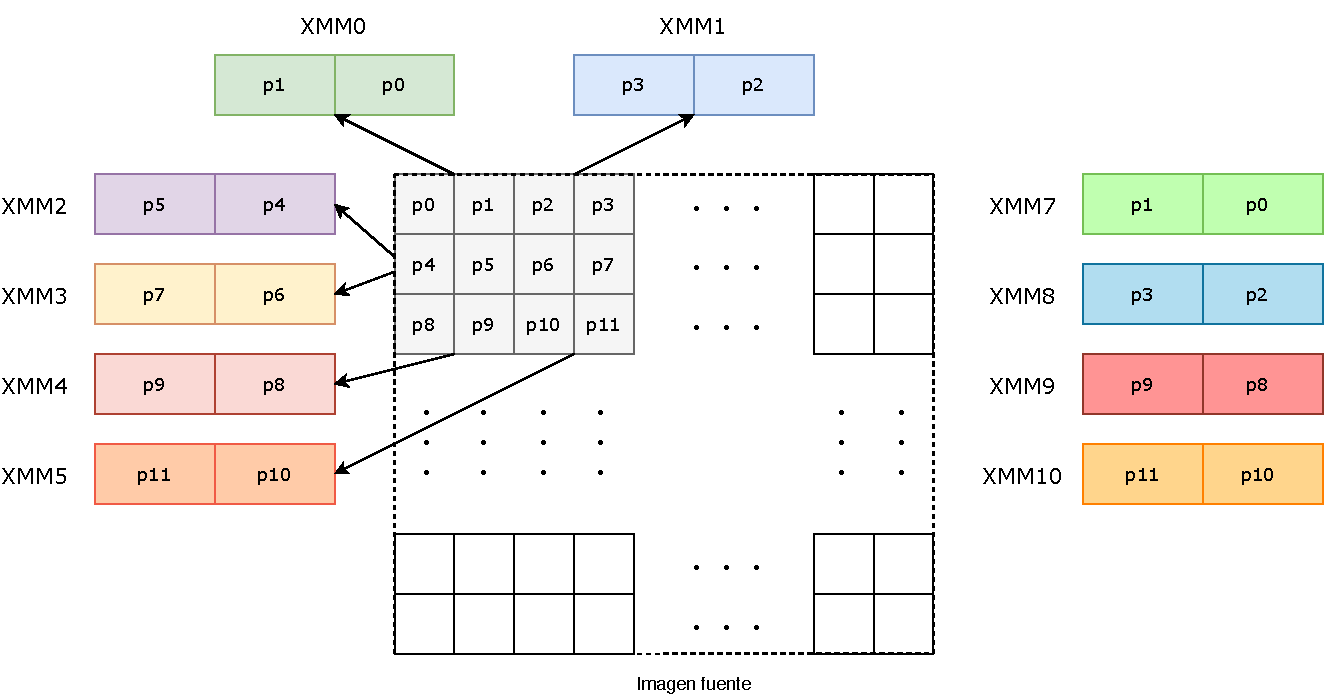
\includegraphics[scale=0.6]{img/LevColorBordes.pdf}
	\end{center}
	
	Para calcular las diferencias horizontales, se restan los registros correspondientes a una misma fila y luego se toma valor absoluto. El resultado de cada diferencia calculada se suma al registro xmm6, acumulándose en la parte alta la suma de diferencias horizontales para el píxel de la posición [rdi + 4] (píxel 6 en el ejemplo) y en la parte baja la suma de diferencias horizontales para el píxel de la posición [rdi] (p5 en el ejemplo).
	
	\begin{center}
		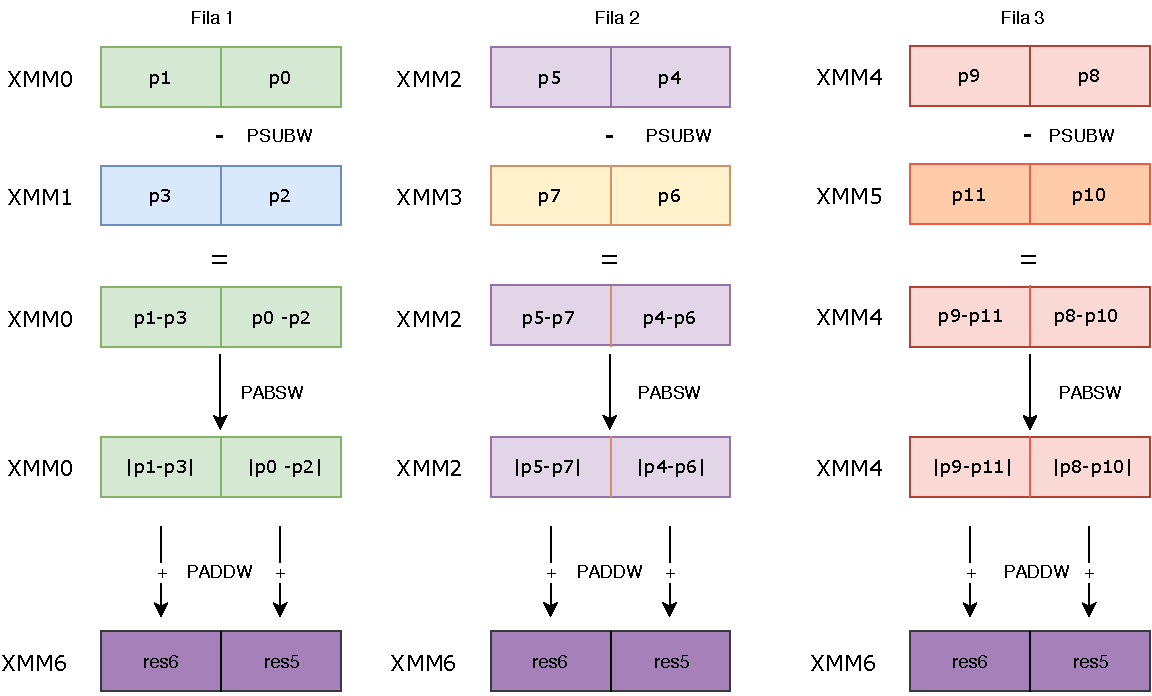
\includegraphics[scale=0.6]{img/sumHorizontalColorBordes.pdf}
	\end{center}

	Para calcular las diferencias verticales, se restan los registros correspondientes al mismo par de columnas, se toma valor absoluto y se suman a xmm6. En este caso, las diferencias verticales de las columnas 2 y 3 deben ser sumadas tanto a la parte alta como a la parte baja del registro xmm6, por lo que es necesario reordenar los resultados para sumar los valores que faltan. \\
	El siguiente esquema muestra gráficamente la operatoria realizada para obtener las sumas de las diferencias verticales:
	
	\begin{center}
		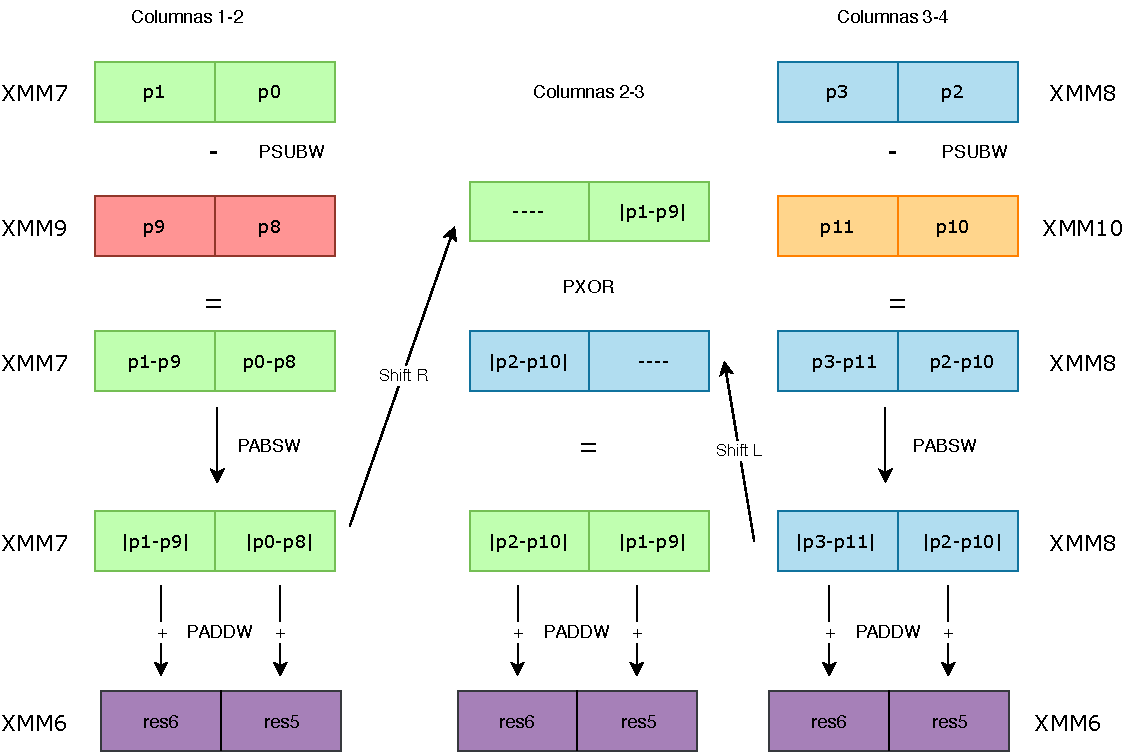
\includegraphics[scale=0.6]{img/sumVerticalesColorBordes.pdf}
	\end{center}
	   
	Luego de acumular en xmm6 las sumas de las diferencias horizontales y verticales, se empaqueta el registro para convertir devuelta a byte y se arreglan las transparencias usando las máscaras destinadas a esto. Hecho esto, se mueven los resultados de los dos píxeles procesados a la imagen destino y se actualizan los índices sumando 8 bytes a rdi y a rsi.
	
	Antes de avanzar de fila, se pinta de blanco el último píxel de la matriz destino, de esta manera se arma el margen vertical derecho de la imagen destino.
	\item \textbf{.bordesUltimaFila}\\
	Este ciclo realiza la misma operatoria que .bordesPrimeraFila, pero usa como registro contador a \textbf{r10d} y como registro índice a \textbf{edx}, que terminó con el valor 0 luego del primer ciclo bordes.
\end{itemize}
	



   
\subsubsection{Reforzar Brillo}

\justify
Nuevamente se definieron en primer lugar las máscaras a utilizar en la operatoria con los píxeles, estas son:
\begin{itemize}
	\item \textit{transparencia}: máscara utilizada para borrar la componente de transparencia del píxel, la misma fue luego arreglada al terminar el ciclo usando la máscara \textit{fix}.
	\item \textit{green}: máscara utilizada para extraer la componente G del píxel, ya que es la única componente que duplica su valor al calcularse el brillo.
	\item \textit{fix}: máscara utilizada para fijar el valor de las transparencias de los píxeles al valor de 255.
\end{itemize} 
\justify
Previo a comenzar el ciclo, dichas máscaras fueron guardadas en los registros \textit{xmm15, xmm14 y xmm9}, respectivamente. Además se guardaron el UmbralSup, el UmbralInf, el BrilloSup y el BrilloInf en los registros \textit{xmm13, xmm12, xmm11 y xmm10}. Se realizó el broadcasting necesario en dichos registros y, en el caso de los brillos, se empaquetaron en 8 bits teniendo en cuenta que si el valor era mayor a 255 debía saturarse a ese valor.

La idea principal de este algoritmo es recorrer la imagen levantando de memoria 4 píxeles consecutivos en el registro \textit{xmm4} y utilizando registros auxiliares calcular el brillo de cada píxel y determinar a cuales píxeles se les debe sumar brillo.
 
 %acá va una imagen mostrando el levantamiento de memoria
 
 Más específicamente, en cada iteración del ciclo se realizaron los siguientes pasos:
 
 \begin{enumerate}
 	\item \textbf{Cálculo de brillo}\\
 	Una vez levantados los 4 píxeles en el registro \textit{xmm4} se elimina la transparencia de estos píxeles usadando la mencionada máscara \textit{transparencia} puesto que el componente A no es necesario en el cálculo de brillo. Para efectuar los cálculos propicios se realiza una copia de los valores de \textit{xmm4} en \textit{xmm3}. Posteriormente, se extraen al registro \textit{xmm2} los componentes G de cada píxel utilizando la mascara \textit{green} y se eliminan los componentes G del registro \textit{xmm3}.
 	Para poder realizar el cálculo de brillo correctamente es necesario extender los componentes R, G y B de \textit{byte} a \textit{word} puesto que al realizar las operaciones requeridas los valores resultantes podrían excederse del rango numérico propio del \textit{byte}. Por este motivo los componentes G del \textit{xmm2} son primeramente alineados a \textit{word} y luego multiplicados por 2. Por otro lado, los componentes R y G que se encuentran aún en \textit{xmm3} están alineados ya a \textit{word} por lo que se procede a realizar la suma horizontal de estos dos con el formato de 16 \texit{bits}.
 	Por una cuestión de conveniencia, se desempaquetan las sumas de los componentes R y B de los 4 píxeles que se encuentran en la parte baja de \textit{xmm3} transformándolas de \textit{word} a \textit{dword}.  Gracias a que los valores de 2*G  en \textit{xmm2} están alineados a \texit{dword} procedemos a sumar los valores correspondientes a cada píxel en el formato de 32 \textit{bits}. De esta manera se obtiene en el registro \textit{xmm3} los brillos correspondientes a cada pixel pero multiplicados por 4. Simplemente shifteando a derecha dos veces cada \textit{dword} se obtienen finalmente los 4 brillos definidos en la operación: 
 	 \begin{equation}
 	B = (src[i][j].r + 2 * src[i][j].g + src[i][j].b)/4 
 	\end{equation}
 	 
 
 	\item \textbf{Adición de brillo superior}\\
 	
	Una vez calculados los 4 brillos se transfieren al registro \textit{xmm6} donde luego son comparados uno a uno con los valores de umbral superior guardados en \textit{xmm13}. En caso de que un brillo sea mayor al umbral superior, se guarda en \textit{xmm6} en los 32 \textit{bits} correspondientes una máscara con 1s. Caso contrario se guarda en esa posición una máscara con 0s. Con ayuda de estas máscaras y utilizando los valores guardados en \textit{xmm11} se colocan en \textit{xmm6} 4 brillos superiores en los 32 \textit{bits} donde correspondan. Finalmente se suman \textit{byte} a \textit{byte} los registros \textit{xmm4} y \texit{xmm6}.
 	
 	\item \textbf{Adición de brillo inferior}\\
 	
 	Para realizar la adición del brillo inferior, se transfieren ahora a \textit{xmm6} los umbrales inferiores guardados en \textit{xmm12} para que luego sean comparados uno a uno con los brillos de cada píxel. De manera análoga a la anterior, en caso de que un umbral inferior sea mayor al brillo se guarda en esa posición una máscara con 1s, y en el caso contrario con 0s. Nuevamente con ayuda de estas máscaras y ahora utilizando los valores de brillo inferior guardados en \textit{xmm13} se colocan en \textit{xmm6} 4 brillos inferiores en los 32 \textit{bits} donde correspondan. Luego se restan \textit{byte} a \textit{byte} los registros \textit{xmm4} y \texit{xmm6}.
 	
 	En último lugar se arreglan las transparencias de los píxeles con la máscara \textit{fix} y se cargan los 4 pixeles a la imagen Destino.
 	    
 \end{enumerate}
 
	
\end{itemize}	 

\subsection{Comparación entre implementaciones en ASM y C}

\subsection{Diseño experimental}



\section{Resultados}
%\input{enunciado}

\section{Conclusión}


\end{document}

